\documentclass{article}

\usepackage{fancyhdr}
\usepackage{extramarks}
\usepackage{amsmath}
\usepackage{amsthm}
\usepackage{amsfonts}
\usepackage{hyperref}
\usepackage{tikz}
\usepackage{tikz-cd}
\usepackage[plain]{algorithm}
\usepackage{algpseudocode}
\usepackage{graphicx}


\newcommand{\R}{\mathbb R}
\newcommand{\N}{\mathbb N}
\newcommand{\Z}{\mathbb Z}
\newcommand{\C}{\mathbb C}
\newcommand{\Q}{\mathbb Q}
\newcommand{\Hb}{\mathbb H}
\newcommand{\defeq}{\vcentcolon=}
\newcommand{\sep}{\ensuremath{.\,}}

\DeclareMathOperator*{\im}{im}
\DeclareMathOperator*{\id}{id}
\DeclareMathOperator*{\ann}{Ann}
\DeclareMathOperator*{\spec}{Spec}
\DeclareMathOperator*{\ob}{Ob}

\newcommand{\E}{\mathrm{E}}
\newcommand{\Var}{\mathrm{Var}}
\newcommand{\Cov}{\mathrm{Cov}}
\newcommand{\Bias}{\mathrm{Bias}}
\renewcommand{\phi}{\varphi}

\newtheorem{definition}{Definition}[section]
\newtheorem{example}{Example}[section]
\newtheorem{lemma}{Lemma}[section]

\begin{document}
    \title{Coalgebras for a functor}
    \maketitle
    \begin{definition}[Algebra]
        \(S\) a category, \(F:S\to S\) an andofunctor.
        
        \(F\)-algebra is an object \(A\in \ob S\) with an arrow \(\alpha: F(A)\to A\). 
    \end{definition}
    \begin{definition}[Coalgebra for an endofunctor]
        \(S\) a category, \(F:S\to S\) an endofunctor.

        \(F\)-coalgebra is an object \(X\in \ob S\) with an arrow \(\alpha: X\to F(X)\).

        We denote it \((X, \alpha: X\to FX)\)
    \end{definition}
    \begin{definition}[Coalgebra homomorphism]
        \(S\) category, \(F:S\to S\) endofunctor, \((x,\alpha: x\to Fx)(y,\beta:y\to Fy)\) coalgebras

        A coalgebra homomorphism \(f:(x,\alpha)\to (y,\beta)\) is a morphism \(f:x\to y\) in S where
        \begin{align*}
            \beta\circ f = F(f)\circ \alpha 
        \end{align*}
        \begin{center}
            \begin{tikzcd}
                x \arrow[d, "\alpha"] \arrow[r, "f"] & y \arrow[d, "\beta"] \\
                F(y) \arrow[r, "F(f)"]               & F(y)                
            \end{tikzcd}
        \end{center}
    \end{definition}
    Coalgebras form a category. Objects are coalgebras, arrows are homomorphisms.

    \section{Polynomial functor}
    A \href{https://ncatlab.org/nlab/show/polynomial+functor}{polynomial} in a (\href{https://ncatlab.org/nlab/show/locally+cartesian+closed+category}{nice}) category is a diagram of the form
    \begin{center}
        \begin{tikzcd}
            x & y \arrow[l, "f"'] \arrow[r, "g"] & z \arrow[r, "h"] & w            
        \end{tikzcd}
    \end{center}
    The corresponding polynomial functor is a composition of functors in the diagram
    \begin{center}
        \begin{tikzcd}
            C/x \arrow[r, "f^*"] & C/y \arrow[r, "\prod_g"] & C/z \arrow[r, "\sum_h"] & C/w            
        \end{tikzcd}
    \end{center}
    where \(/\) denotes slice categories, \(\prod_g\) is right adjoint to \(g^*\), \(\sum_h\) left adjoint to \(h^*\), \((-)^*\) are pullback functors. In Set, \(f\) and \(h\) are terminal maps.

    \begin{definition}[polynomial functors in Set]
        Given a function \(g:X\to Y\), a polynomial functor is a functor
        \begin{align*}
            p:Set\to Set\\
            p:S\mapsto \coprod_{y\in Y} \{f:g^{-1}(y)\to S\}
        \end{align*}
        Or equivalently
        \begin{align*}
            p:S\mapsto \coprod_{y\in Y}S^{X_y}
        \end{align*}
    \end{definition}
    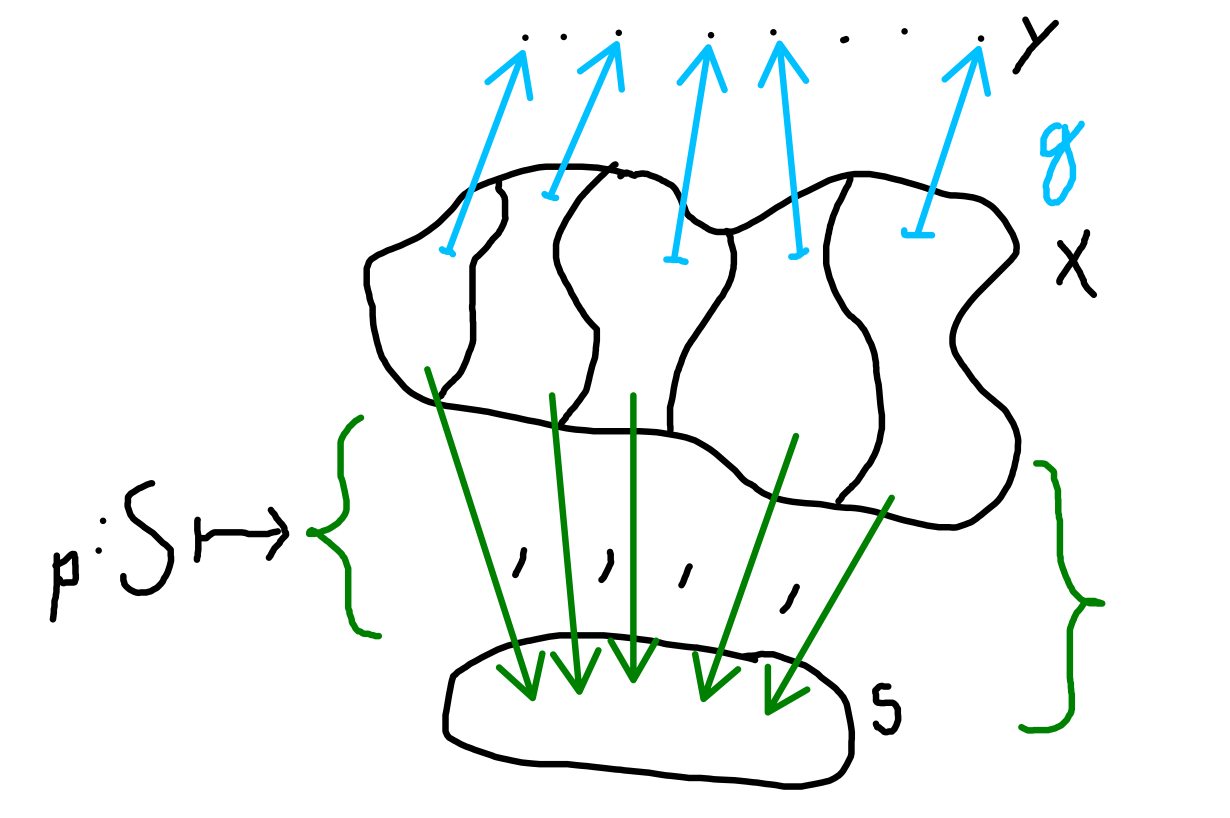
\includegraphics[width=0.8\textwidth]{polyf}

    I also present Awodey's definition:
    \begin{definition}[Polynomial functors in Set]
        A polynomial functor \(p\) is a functor 
        \begin{align*}
            p:Set\to Set\\
            p:S\mapsto \coprod_{j\in\Gamma} C_j \times S^{B_j}
        \end{align*}
        If \(\Gamma\) is finite and \(B_j\)'s and \(C_j\)'s are finite, we get a familiar notion of a polynomial.
    \end{definition}
    
    \begin{definition}[final coalgebra]
        The terminal object in the category of F-Coalgebras.
    \end{definition}

    Polynomial functors preserve colimits

    \begin{example}
        The terminal object for \(p\)-Coalgebras are \(M\) types --- trees. An element from the terminal object is a specific tree, where each node has a carrier set \(C_i\) and children indexed by \(B_i\). The children are again, nodes.

        Build such trees coinductively, because they are not necessarily well-founded.
    \end{example}
    \begin{proof}

    \end{proof}
        
\end{document}